\documentclass[12pt,a4paper]{article}

\usepackage[margin=1in]{geometry}
\usepackage[T1]{fontenc}
\usepackage[utf8]{inputenc}
\usepackage{lmodern}
\usepackage{graphicx}
\usepackage{booktabs}
\usepackage{array}
\usepackage{float}
\usepackage{caption}
\usepackage{subcaption}
\usepackage{hyperref}
\usepackage{xcolor}
\usepackage{enumitem}
\usepackage{titlesec}
\usepackage{amsmath}

\hypersetup{
    colorlinks=true,
    linkcolor=blue!50!black,
    urlcolor=blue!60!black,
    citecolor=blue!50!black
}

\titleformat{\section}{\large\bfseries\color{blue!40!black}}{\thesection}{0.75em}{}
\titleformat{\subsection}{\normalsize\bfseries\color{blue!30!black}}{\thesubsection}{0.75em}{}

\title{\textbf{Advanced Spam Email / SMS Detection}\\[0.5em]
\large A Hybrid Machine Learning and NLP Approach}
\author{Project Report}
\date{\today}

\begin{document}

\begin{titlepage}
    \centering
    \vspace*{2.5cm}

    {\Huge \textbf{Advanced Spam Email / SMS Detection}\par}
    \vspace{0.6cm}
    {\Large A Hybrid Machine Learning and NLP Approach\par}
    \vspace{1.8cm}

    {\large Professional Project Report\par}
    \vspace{1.2cm}

    \begin{tabular}{rl}
        \textbf{Project Type:} & Machine Learning / Natural Language Processing \\
        \textbf{Implementation:} & Python Notebook Pipeline \\
        \textbf{Core Models:} & TF-IDF, Logistic Regression, BERT, XGBoost \\
        \textbf{Artifacts:} & Trained vectorizer and saved model files \\
    \end{tabular}

    \vfill

    {\large
    Repository notebook: \texttt{advance\_spam\_detection\_BTP.ipynb}\par
    }
    \vspace{0.5cm}
    {\large
    Colab link: \href{https://colab.research.google.com/drive/1PKJwAwZ50F5eHQ_Dw-dc7CqMyFmJ_XWa?usp=sharing}{Open Notebook}
    \par}

    \vfill

    {\large \today\par}
\end{titlepage}

\tableofcontents
\newpage

\section{Abstract}
This project presents a spam-message detection workflow that progresses from a classical text-classification baseline to a stronger hybrid model using modern natural language processing features. The system begins with TF-IDF and Logistic Regression, extends the representation with handcrafted message-level indicators, and then incorporates BERT embeddings with XGBoost for richer semantic modeling. Additional steps include probability calibration, threshold tuning, SHAP-based interpretation, and a graph-inspired feature experiment. The reported results show that the hybrid approach substantially improves spam identification while maintaining strong overall accuracy, reaching a reported ROC-AUC of 0.9967 on the held-out test set.

\section{Introduction}
Spam detection remains a practical and important classification problem in email and SMS systems. A useful spam filter should not only detect suspicious messages accurately, but also avoid incorrectly flagging legitimate communication. This project explores how performance changes as the feature representation becomes more expressive.

The notebook is structured as a full machine learning story:
\begin{itemize}[leftmargin=1.5em]
    \item exploratory data analysis,
    \item baseline model training,
    \item richer feature engineering,
    \item hybrid model design,
    \item evaluation and interpretation.
\end{itemize}

\section{Dataset Description}
The project uses a public SMS spam dataset containing \textbf{5,572 messages}. Each message is labeled as either:
\begin{itemize}[leftmargin=1.5em]
    \item \textbf{ham} for legitimate messages, or
    \item \textbf{spam} for unwanted/promotional/fraudulent messages.
\end{itemize}

The notebook reports the following split:
\begin{itemize}[leftmargin=1.5em]
    \item \textbf{Training samples:} 4,457
    \item \textbf{Testing samples:} 1,115
\end{itemize}

\subsection{Exploratory Visual Analysis}
The class distribution and text-pattern plots reveal how spam differs from ham messages in both frequency and structure.

\begin{figure}[H]
    \centering
    \begin{subfigure}[t]{0.48\textwidth}
        \centering
        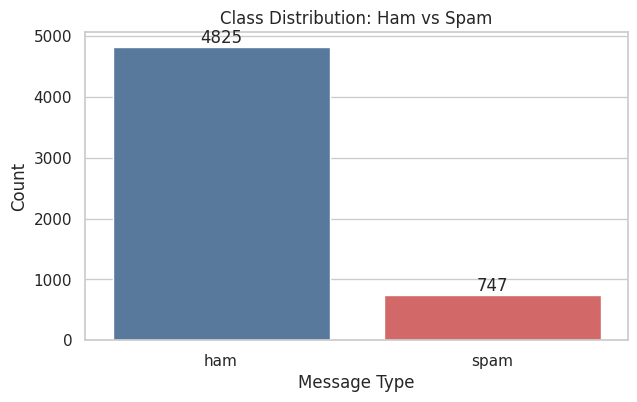
\includegraphics[width=\linewidth]{../assets/output/class_distribution.png}
        \caption{Class distribution of ham and spam messages}
    \end{subfigure}
    \hfill
    \begin{subfigure}[t]{0.48\textwidth}
        \centering
        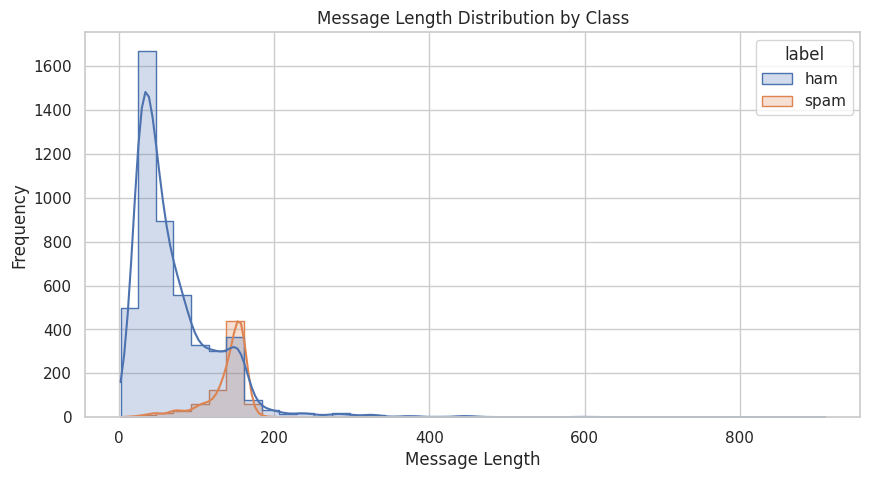
\includegraphics[width=\linewidth]{../assets/output/message_length_distribution.png}
        \caption{Message-length distribution by class}
    \end{subfigure}
    \caption{Initial data exploration}
\end{figure}

\begin{figure}[H]
    \centering
    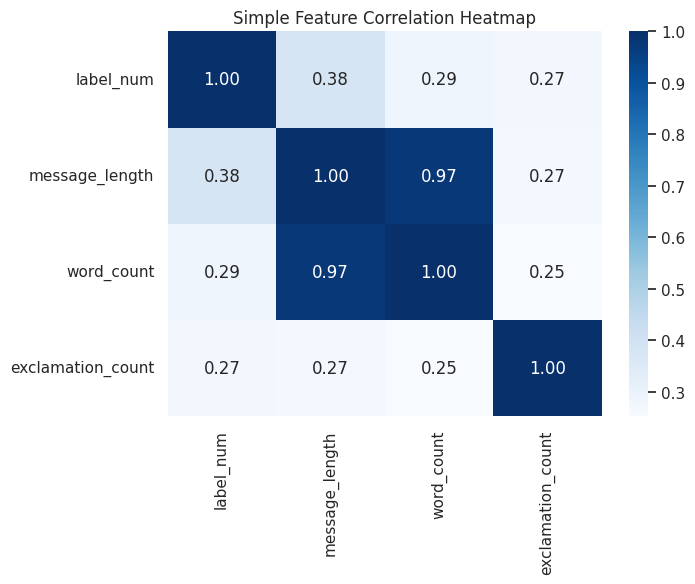
\includegraphics[width=0.62\textwidth]{../assets/output/feature_correlation.png}
    \caption{Correlation among simple engineered features}
\end{figure}

\section{Methodology}
\subsection{Baseline Text Model}
The first stage converts messages into TF-IDF vectors with a feature cap of \textbf{5,000}. A Logistic Regression classifier is then trained on the transformed text. This gives a strong and interpretable baseline for spam detection.

\subsection{Handcrafted Features}
To add lightweight human-intuition signals, the notebook introduces simple numeric features such as:
\begin{itemize}[leftmargin=1.5em]
    \item total character length,
    \item count of exclamation marks,
    \item count of dollar signs.
\end{itemize}
These features are combined with TF-IDF vectors to test whether simple message cues improve performance.

\subsection{BERT-Augmented Hybrid Model}
The next stage uses \texttt{bert-base-uncased} to extract \textbf{768-dimensional} sentence embeddings. These embeddings are concatenated with TF-IDF features, producing a hybrid representation that captures both word importance and semantic context. An XGBoost classifier is trained on this combined feature space.

\subsection{Calibration and Threshold Tuning}
Because classification confidence matters in real spam filtering, the workflow calibrates the model probabilities using sigmoid calibration. Precision-recall analysis is then used to inspect threshold behavior and support high-precision operating points.

\subsection{Interpretability and Error Analysis}
To better understand model behavior, the notebook applies SHAP analysis on a sample of predictions and also inspects misclassified test examples. This strengthens the project by moving beyond accuracy alone and examining why certain mistakes occur.

\subsection{Graph-Inspired Feature Extension}
As a creative extension, the project treats each message as a simple word graph and computes structural properties such as:
\begin{itemize}[leftmargin=1.5em]
    \item number of nodes,
    \item number of edges,
    \item graph density.
\end{itemize}
These graph-style features are appended to the previous representation and evaluated as an experimental enhancement.

\section{Model Results}
The notebook reports the following milestone outcomes on the held-out test set.

\begin{table}[H]
    \centering
    \caption{Performance across model stages}
    \begin{tabular}{>{\raggedright\arraybackslash}p{0.58\textwidth} >{\centering\arraybackslash}p{0.28\textwidth}}
        \toprule
        \textbf{Model Stage} & \textbf{Reported Result} \\
        \midrule
        TF-IDF + Logistic Regression & 97.58\% accuracy \\
        TF-IDF + handcrafted features & 97.04\% accuracy \\
        TF-IDF + BERT + XGBoost & 0.99 accuracy in report, ROC-AUC = 0.9967 \\
        Graph-augmented hybrid model & 98.83\% accuracy \\
        \bottomrule
    \end{tabular}
\end{table}

Additional observations from the notebook:
\begin{itemize}[leftmargin=1.5em]
    \item Best grid-search parameters: \texttt{max\_depth = 4}, \texttt{n\_estimators = 100}
    \item Suggested high-precision threshold: 0.0008
    \item Number of misclassified examples highlighted in analysis: 13
\end{itemize}

\subsection{Comparison and Evaluation Figures}
\begin{figure}[H]
    \centering
    \begin{subfigure}[t]{0.48\textwidth}
        \centering
        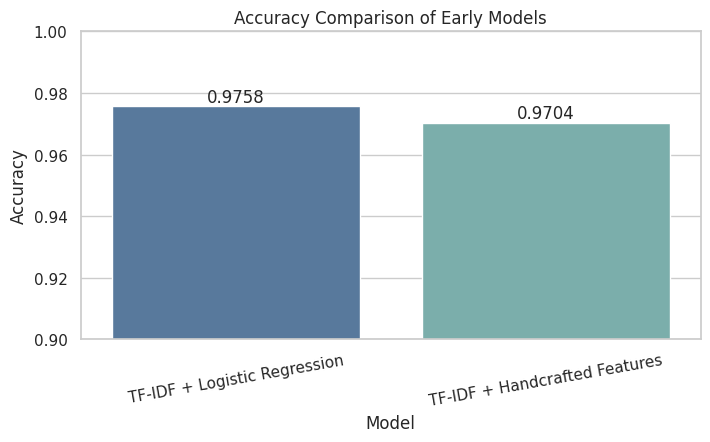
\includegraphics[width=\linewidth]{../assets/output/baseline_vs_handcrafted.png}
        \caption{Baseline versus handcrafted feature model}
    \end{subfigure}
    \hfill
    \begin{subfigure}[t]{0.48\textwidth}
        \centering
        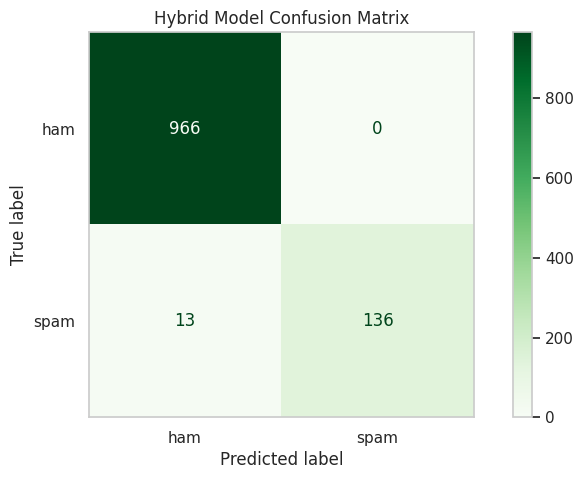
\includegraphics[width=\linewidth]{../assets/output/hybrid_confusion_matrix.png}
        \caption{Confusion matrix of the hybrid model}
    \end{subfigure}
    \caption{Model evaluation visuals}
\end{figure}

\begin{figure}[H]
    \centering
    \begin{subfigure}[t]{0.48\textwidth}
        \centering
        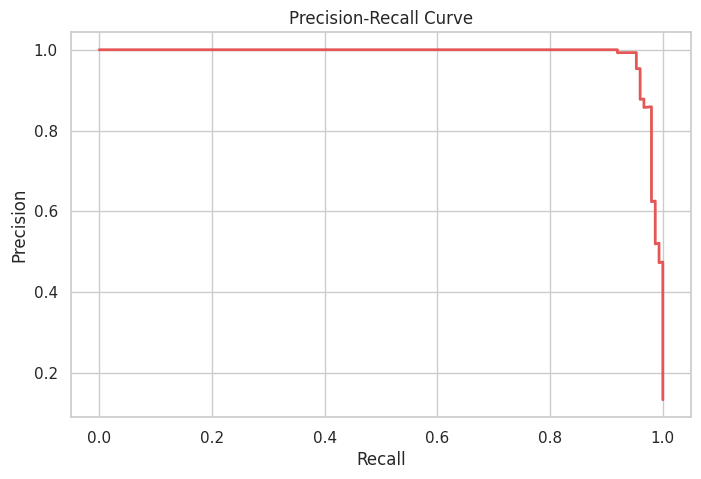
\includegraphics[width=\linewidth]{../assets/output/precision_recall_curve.png}
        \caption{Precision-recall trade-off}
    \end{subfigure}
    \hfill
    \begin{subfigure}[t]{0.48\textwidth}
        \centering
        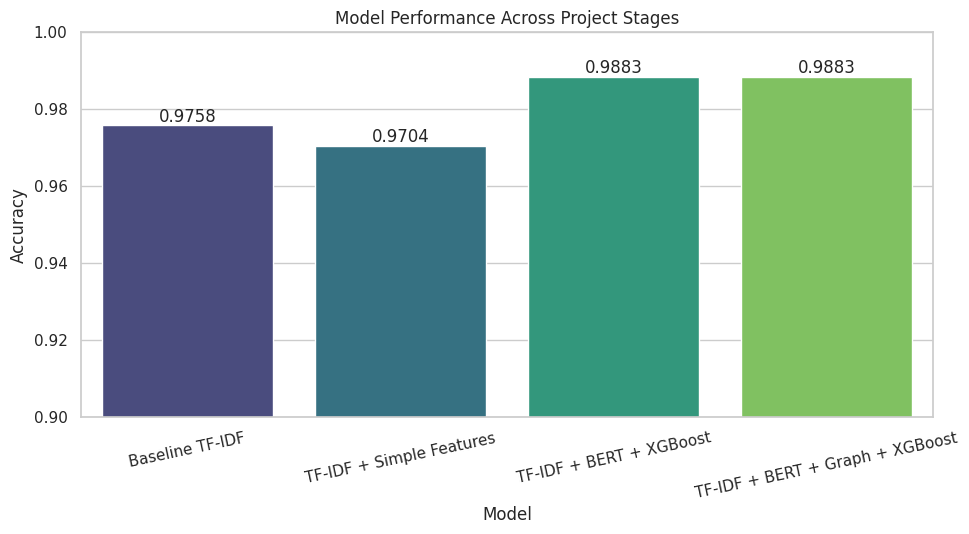
\includegraphics[width=\linewidth]{../assets/output/final_model_comparison.png}
        \caption{Final comparison across model stages}
    \end{subfigure}
    \caption{Final performance summary}
\end{figure}

\section{Model Interpretation}
Interpretability is a valuable component of applied machine learning, especially when the model may be used in communication systems. SHAP analysis helps identify which input features influence predictions the most, offering a clearer view of how the model separates spam from legitimate messages.

\begin{figure}[H]
    \centering
    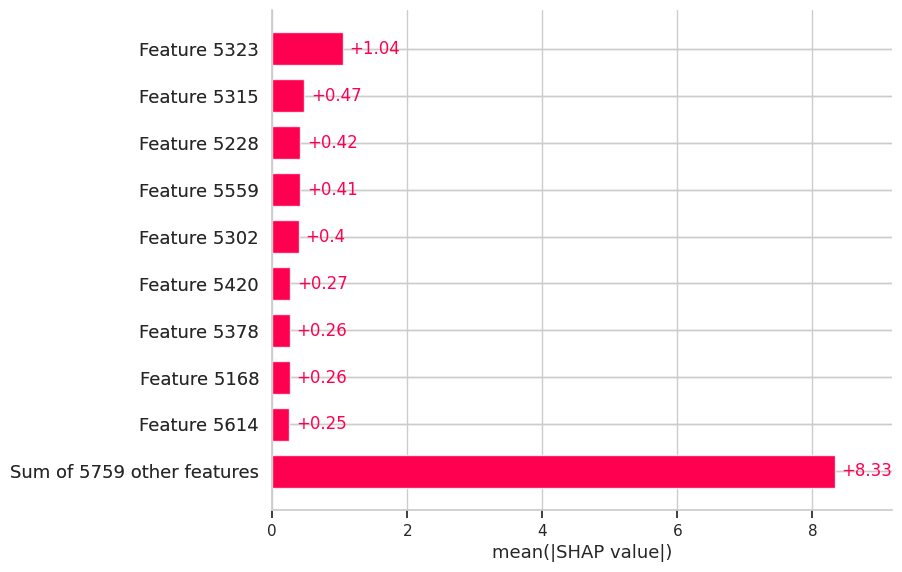
\includegraphics[width=0.72\textwidth]{../assets/output/shap_summary.png}
    \caption{SHAP-based summary of feature influence}
\end{figure}

\section{Saved Artifacts}
The repository currently includes the following saved outputs:
\begin{itemize}[leftmargin=1.5em]
    \item \texttt{tfidf.pkl} for TF-IDF vectorization,
    \item \texttt{spam\_model\_v2.pkl} for the hybrid classifier,
    \item \texttt{spam\_model\_calibrated.pkl} for calibrated probability prediction.
\end{itemize}

One practical limitation is that the notebook's prediction helper expects saved \texttt{bert\_model/} and \texttt{bert\_tokenizer/} directories, which are referenced in the workflow but are not currently present in the repository snapshot.

\section{Discussion}
The project shows a clear progression from a strong classical NLP baseline to a more expressive hybrid pipeline. The TF-IDF model already performs well, which is common for spam datasets with distinctive vocabulary patterns. The addition of BERT embeddings improves the system by providing contextual information that pure bag-of-words methods may miss. Calibration and threshold tuning also make the project more deployment-aware, since spam filtering often values precision and confidence quality as much as raw accuracy.

The graph-inspired extension is an interesting exploratory step. Even if it does not outperform the best semantic hybrid model, it demonstrates creativity in feature design and opens the door to more structural text representations.

\section{Conclusion}
This report presents a complete spam-detection workflow built around progressive modeling, evaluation, and interpretation. The final project combines traditional text vectorization with transformer-based semantic features and gradient-boosted classification, resulting in very strong reported performance. Beyond predictive quality, the notebook also demonstrates good machine learning practice through calibration, visualization, error analysis, and interpretability. Overall, the repository serves both as a practical spam-classification project and as a strong educational example of end-to-end NLP modeling.

\section*{References}
\begin{enumerate}[leftmargin=1.5em]
    \item UCI SMS Spam Collection style dataset as accessed in the notebook from a public TSV source.
    \item Pedregosa et al., \textit{Scikit-learn: Machine Learning in Python}.
    \item Devlin et al., \textit{BERT: Pre-training of Deep Bidirectional Transformers for Language Understanding}.
    \item Chen and Guestrin, \textit{XGBoost: A Scalable Tree Boosting System}.
    \item Lundberg and Lee, \textit{A Unified Approach to Interpreting Model Predictions}.
\end{enumerate}

\end{document}
